\begin{pastexam}[label={px:ncku-114-prog-11}]{成大資訊聯招 114 學年度 第 11 題}
（複選；至少有二個正確答案）

{[4\%]} Considering the following adjacency matrix.
\begin{center}
\begin{tabular}{c|*{8}{c|}}
\multicolumn{1}{c}{} & \multicolumn{1}{c}{0} & \multicolumn{1}{c}{1} & \multicolumn{1}{c}{2} & \multicolumn{1}{c}{3} & \multicolumn{1}{c}{4} & \multicolumn{1}{c}{5} & \multicolumn{1}{c}{6} & \multicolumn{1}{c}{7} \\ \cline{2-9}
0 &   &   &   &   & 1 &   & 1 &   \\ \cline{2-9}
1 &   &   & 1 &   &   & 1 &   &   \\ \cline{2-9}
2 &   & 1 &   &   &   & 1 &   &   \\ \cline{2-9}
3 &   &   &   &   & 1 &   & 1 &   \\ \cline{2-9}
4 & 1 &   &   & 1 &   &   &   &   \\ \cline{2-9}
5 &   & 1 & 1 &   &   &   &   & 1 \\ \cline{2-9}
6 & 1 &   &   & 1 &   &   &   &   \\ \cline{2-9}
7 &   &   &   &   &   & 1 &   &   \\ \cline{2-9}
\end{tabular}
\end{center}
\smallskip
Please reconstruct the undirected graph based on the above adjacency matrix. Which of the following statements related to the resultant graph are correct?
\begin{enumerate}[label=(\Alph*)]
\item The breath-first search starting at vertex 1 produces a spanning tree with 8 vertices.
\item The degree of vertex 4 is 2.
\item The graph has one articulation point.
\item The graph has one connected component.
\item The graph has two cycles.
\end{enumerate}
\end{pastexam}

\begin{pastsoln}
答案：(B)、(C)、(E)。

\textbf{還原圖}（資結書第~21.2~節）。 矩陣是對稱的，第 $i$ 列第 $j$ 欄是 $1$ 就有無向邊 $(i, j)$：
\[
(0, 4),\ (0, 6),\ (1, 2),\ (1, 5),\ (2, 5),\ (3, 4),\ (3, 6),\ (5, 7),
\]
共 $8$ 條邊。 分成兩個連通塊：
\begin{itemize}
\item $\{0, 3, 4, 6\}$：$0$--$4$--$3$--$6$--$0$，一個長度 $4$ 的環。
\item $\{1, 2, 5, 7\}$：$1$--$2$--$5$--$1$ 是長度 $3$ 的環，$7$ 只接在 $5$ 上。
\end{itemize}
\begin{center}
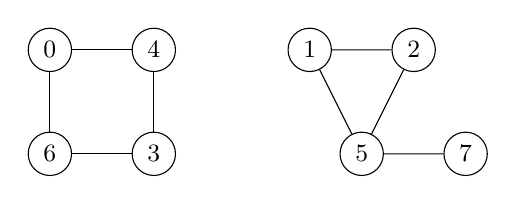
\begin{tikzpicture}[x=1.1cm,y=1.1cm,v/.style={circle,draw,inner sep=0pt,minimum size=5.5mm,font=\small}]
\node[v] (0) at (0,0) {0}; \node[v] (4) at (1.2,0) {4}; \node[v] (3) at (1.2,-1.2) {3}; \node[v] (6) at (0,-1.2) {6};
\draw (0)--(4)--(3)--(6)--(0);
\node[v] (1) at (3,0) {1}; \node[v] (2) at (4.2,0) {2}; \node[v] (5) at (3.6,-1.2) {5}; \node[v] (7) at (4.8,-1.2) {7};
\draw (1)--(2)--(5)--(1) (5)--(7);
\end{tikzpicture}
\end{center}

逐項檢查：
\begin{itemize}
\item (A) 錯。 從 $1$ 做 BFS 只走得到同一個連通塊的 $1, 2, 5, 7$，得到的生成樹只有 $4$ 個頂點；圖不連通，沒有 $8$ 個頂點的生成樹。
\item (B) 對。 第 $4$ 列有兩個 $1$（第 $0$、$3$ 欄），度數 $2$。
\item (C) 對。 拿掉 $5$ 以後 $7$ 和 $1$、$2$ 分開，$5$ 是割點（資結書第~23.5~節）。 其他頂點都不是：$4$ 個點的環拿掉任一點仍連通；
$1$、$2$ 拿掉後剩下的仍連在 $5$ 上；$7$ 是葉子。 只有一個割點。
\item (D) 錯。 有兩個連通塊。
\item (E) 對。 兩個連通塊裡各有一個環：$0$--$4$--$3$--$6$--$0$ 和 $1$--$2$--$5$--$1$。 每個連通塊都是 $4$ 個頂點、$4$ 條邊；
連通圖的邊數等於頂點數時，比樹多一條邊，恰好有一個環，所以全圖就是這兩個環。
\end{itemize}
\end{pastsoln}
